\section{Controller Analysis}\label{ssec:ControllerVerification}
A further analysis can be done to the controller, both continuous and discrete, and also to the real response of the system once it is implemented.

The first step is to simulate both the continuous and discrete controller with the model of the system and analyse the behavior of the whole closed loop system.

This is done not only to see the behavior of the designed controller but also to verify that the discretized controller matches the original continuous one. 

With a constant reference of 0 rad and a disturbance in the form of a torque applied to the frame of \si{0,55 Nm}, the responses are the ones shown in \figref{discreteVsContinuousOutputController} and \figref{discreteVsContinuousSimulation}.
%
\begin{minipage}{0.45\linewidth}
	\begin{figure}[H]
      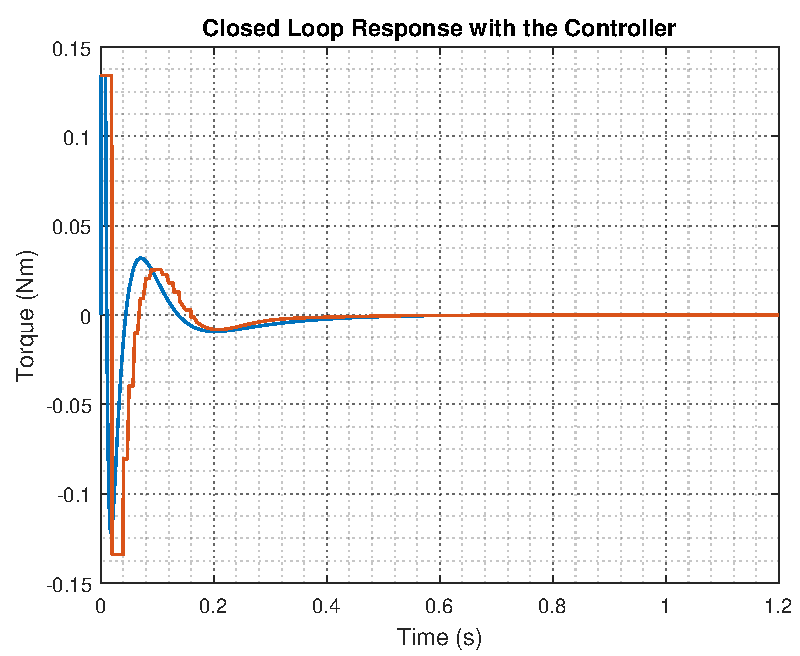
\includegraphics[scale=.53]{figures/torqueComp}
      \captionsetup{justification=centering}
      \captionof{figure}{Controller's output (torque) response in the control loop with the continuous (blue) and discrete (red) controllers}
      \label{discreteVsContinuousOutputController}
    \end{figure}\vspace{-5mm}
\end{minipage}
\hspace{0.03\linewidth}
\begin{minipage}{0.45\linewidth}
    \begin{figure}[H]\vspace{-4mm}
      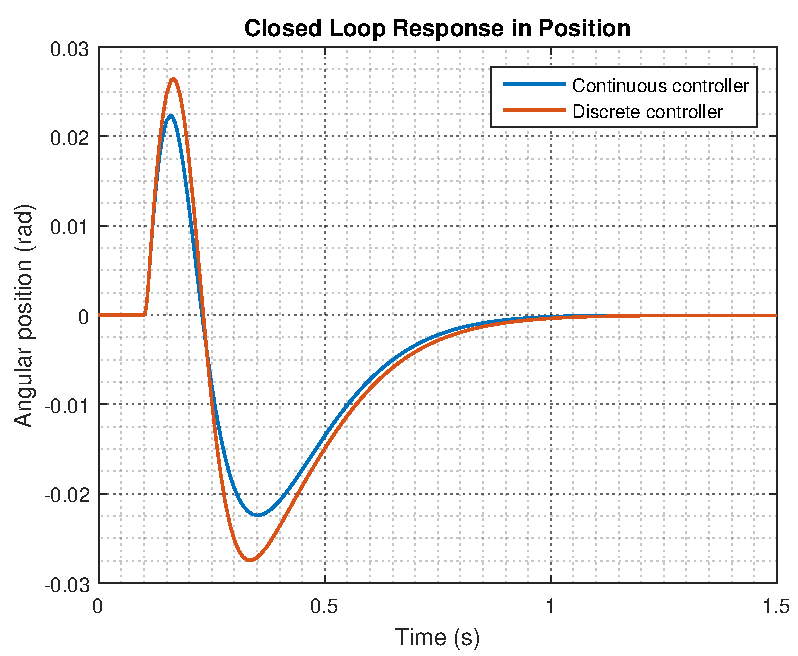
\includegraphics[scale=.53]{figures/positionComp}
      \captionsetup{justification=centering}
      \captionof{figure}{Closed loop response of the continuous (blue) and discrete (red) controllers}
      \label{discreteVsContinuousSimulation}
    \end{figure}\vspace{-5mm}
\end{minipage}

Both controllers seem to have a good behavior and both reach the desired final position. However it is important to look also to the velocity of the wheel, since it has been assumed to be 0 in the equilibrium position.
%
\begin{figure}[H]\vspace{-4mm}
	\centering
	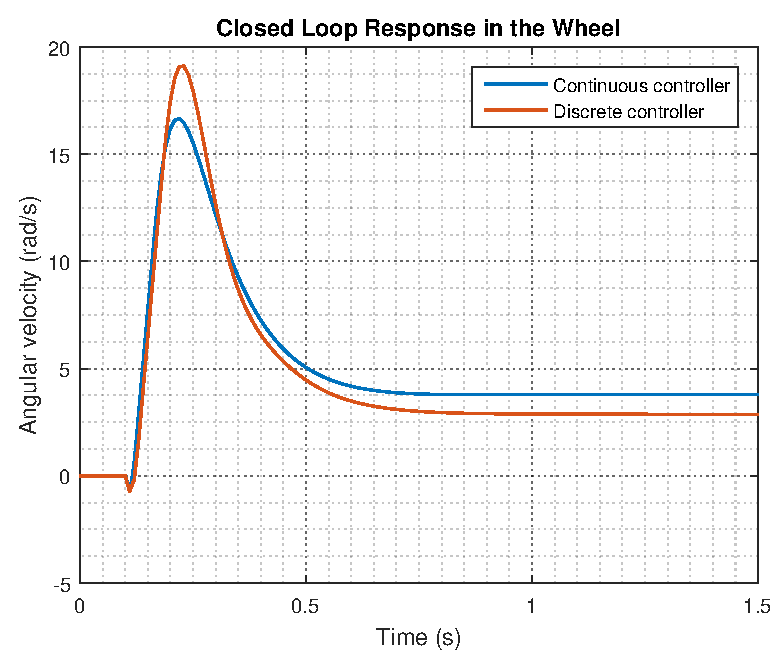
\includegraphics[scale=.53]{figures/wheelComp}
	\captionof{figure}{Angular velocity of the wheel}
   \label{fig:discreteVsContinuousWheel}
\end{figure}\vspace{-5mm}

In both cases the velocity is different from 0 in steady state, with means that the Cubli is not in the equilibrium position defined for it. 

The conclusion of the simulation is that the controller is not able to maintain the system in equilibrium position. This means that another kind of controller in needed, which also takes care of the velocity of the wheel. Since now the system will have two outputs it is reasonable to consider a State Space approach to solve the problem.

Moreover, the response of the real Cubli with the controller can also be tested (see \appref{app:sisoToolDControllerTest}). The torque requested by the controller and the position of the frame are shown in \figref{torqueTustinPre} and \figref{positionTustinPre}.

\begin{minipage}{0.45\linewidth}
	\begin{figure}[H]
		\centering
		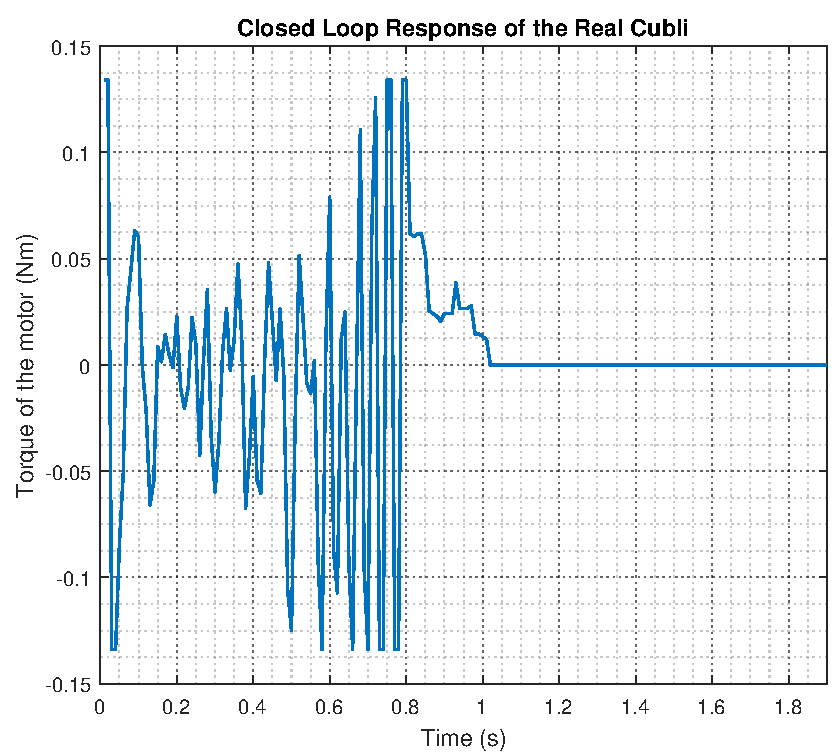
\includegraphics[scale=.53]{figures/torqueTestTustinPre}
		\captionsetup{justification=centering}
		\captionof{figure}{Torque requested by the controller}
		\label{torqueTustinPre}
	\end{figure}\vspace{-5mm}
\end{minipage}
\hspace{0.03\linewidth}
\begin{minipage}{0.45\linewidth}
	\begin{figure}[H]\vspace{-0mm}
		\centering
		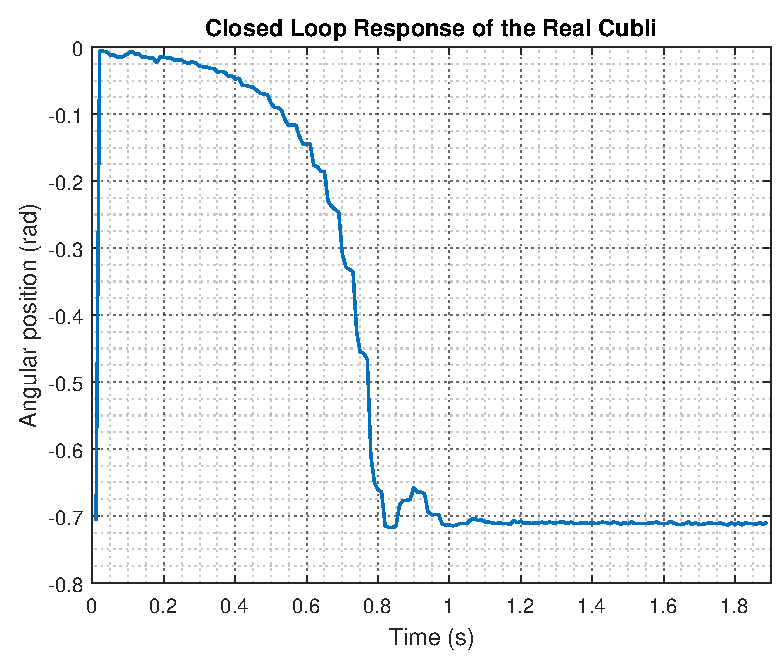
\includegraphics[scale=.53]{figures/positionTestTustinPre}
		\captionsetup{justification=centering}
		\captionof{figure}{Angular position of the Cubli}
		\label{positionTustinPre}
	\end{figure}\vspace{-5mm}
\end{minipage}

 In that case the Cubli starts form equilibrium position and no disturbance is applied to it. Initially the torque should be very low since the error is almost 0. However its value is very high, which makes
 the Cubli fall. 
 

